\documentclass{report}


\usepackage{graphicx} % Required for inserting images
\usepackage{amsmath,amssymb}
\usepackage[ruled,vlined]{algorithm2e}

\usepackage{url}

\usepackage{pgfplots}
\pgfplotsset{compat=1.18} % Use a recent compatibility version
\usetikzlibrary{arrows.meta} % For nicer arrows


\usepackage{xcolor}
\usepackage{listings}


\usepackage[colorlinks=true,
            urlcolor=maincolor]{hyperref}


\definecolor{maincolor}{HTML}{1E90FF}


\definecolor{vscodeBlue}{RGB}{4,100,179}       % keywords
\definecolor{vscodeRed}{RGB}{170,0,0}      % strings
\definecolor{vscodeGreen}{RGB}{0,128,0}      % comments
\definecolor{vscodeDarkYellow}{RGB}{242,134,29} % function names / identifiers
\definecolor{vscodePurple}{RGB}{0,0,110}   % numbers

% Setup listings for Python
\lstset{
    language=Python,
    keywordstyle=\color{vscodeBlue}\bfseries,
    stringstyle=\color{vscodeRed},
    commentstyle=\color{vscodeGreen}\itshape,
    identifierstyle=\color{vscodeDarkYellow},
    numbers=left,
    numberstyle=\tiny\color{gray},
    numbersep=5pt,
    backgroundcolor=\color{white},  % white background
    showstringspaces=false,
    basicstyle=\ttfamily\small,
    breaklines=true,
    frame=tb,
}


\begin{document}

\section{Cifrari Antichi - Cesare}

Cominciamo ad analizzare i primi cifrari, iniziando dal più antico mai inventato: infatti, come avevamo già detto nell'introduzione, il \textbf{Cifrario di Cesare} risale all'Impero romano.  
Il cifrario fu ideato per inviare ai legionari informazioni per proseguire la battaglia.  
Chiaramente non potevano mandare i messaggi in chiaro, anche perché, se gli avversari ne venivano a conoscenza, potevano rispondere con una contromossa.  
Per questo \textbf{Giulio Cesare} inventò un cifrario che si basava sullo spostamento di un determinato numero di posizioni delle lettere nell'alfabeto.  
Un classico esempio del cifrario di Cesare è quello di \textbf{spostare di 3 posizioni indietro}.


\begin{figure}[h]
    \centering
    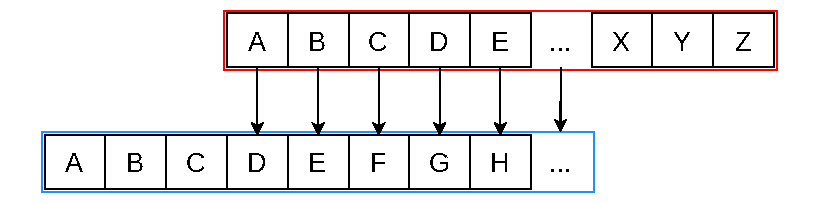
\includegraphics[width=\linewidth]{logos/1_1_cripto.pdf}
\end{figure}


Le lettere che "escono a sinistra" le associamo alle ultime tre lettere.


\begin{figure}[h]
    \centering
    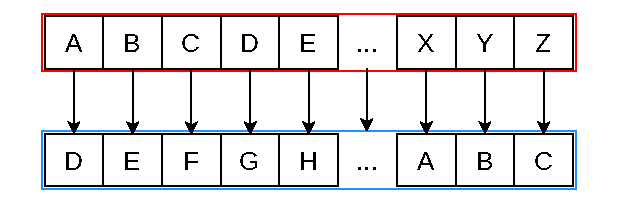
\includegraphics[width=0.8\linewidth]{logos/1_2_cripto.pdf}
\end{figure}

Per cifrare un messaggio basta prendere ogni lettera del testo in chiaro e sostituirla con la lettera corrispondente nella tabella.  
Ad esempio, se volessimo cifrare la parola \textbf{Abbecce}, con il cifrario di Cesare diventerebbe \textbf{Deehffh}.


Per decifrare, invece, basta applicare lo stesso procedimento, ma spostando l'alfabeto verso destra.  
Con questo esempio, il testo decifrato sarà:

\begin{figure}[h]
    \centering
    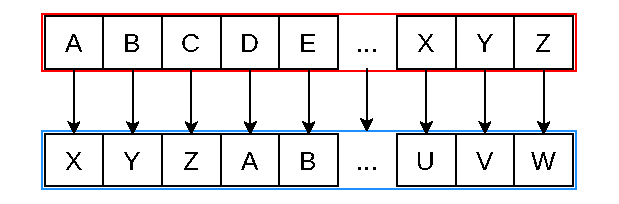
\includegraphics[width=0.8\linewidth]{logos/1_3_cripto.pdf}
\end{figure}


\newpage

In questo esempio abbiamo spostato l'alfabeto di tre posizioni, ma questo è un numero che possiamo scegliere liberamente.  
Secondo la tradizione, Giulio Cesare utilizzava il numero tre, ma si può scegliere qualsiasi valore di spostamento.  
Poiché questo numero è decisivo per la cifratura, il numero di spostamenti non è altro che la \textbf{chiave} del sistema.  
Chiaramente, a chiavi diverse corrispondono cifrari diversi e, di conseguenza, differenti cifrature dei messaggi.


Una possibile implementazione in Python del cifrario di Cesare con 3 spostamenti:

\begin{lstlisting}[language=Python]
def Cifratura_Cesare(mess):
    return "".join([chr(((ord(char) - ord('a') + 3) % 26) + ord('a')) for a in mess])

def Decifratura_Cesare(mess):
    return "".join([chr(((ord(char) - ord('a') - 3) % 26) + ord('a')) for a in mess])
\end{lstlisting}


Online, questa cifratura viene anche chiamata \textbf{ROT} (abbreviazione di \textit{ROTation}), seguita dal numero di spostamenti.  
Quindi, \textbf{ROT3} corrisponde a 3 spostamenti (come negli esempi precedenti), mentre \textbf{ROT15} sposterà di 15 posizioni.  
In Python, un'implementazione per un generico \textbf{ROT-n} potrebbe essere:


\begin{lstlisting}[language=Python]
def Cifratura_ROTn(mess, n):
    return "".join([chr(((ord(char) - ord('a') + n) % 26) + ord('a')) for a in mess])

def Decifratura_ROTn(mess, n):
    return "".join([chr(((ord(char) - ord('a') - n) % 26) + ord('a')) for a in mess])
\end{lstlisting}




Quindi, se qualcuno vuole usare questo cifrario, basta scegliere un numero tra 1 e 25 e tenerlo segreto.  
Tuttavia, questo metodo è soggetto ad attacchi \textbf{brute-force}: come abbiamo detto, questo cifrario ha al massimo \textbf{25 chiavi possibili}, quindi qualcuno potrebbe creare un programma che provi tutte le combinazioni.  
Un possibile programma in Python:


\begin{lstlisting}[language=Python]
def attacco_rotn(messDaDecifrare):
    for i in range(1, 26):
        print(Decifratura_ROTn(messDaDecifrare, i))
\end{lstlisting}


\newpage

\subsection{Cifrari Monoalfabetici}
In realtà, l'attacco brute-force non è l'unico al quale è soggetto questo cifrario.  
Questo tipo di cifrario è definito \textbf{monoalfabetico} perché la stessa lettera viene sempre cifrata con la stessa lettera corrispondente.  
Tutti i cifrari monoalfabetici sono soggetti ad attacchi detti \textbf{Letter Frequency}.  
Ciò significa che la \textbf{percentuale} di una lettera nel testo originale è la stessa della lettera corrispondente nel testo cifrato.  
Facciamo un esempio con \textbf{Abbcccdddd}, che, cifrato con ROT3, diventa \textbf{Deefffgggg}.

\vspace{0.2cm}
\[
\begin{array}{c@{\hskip 0.1cm}c@{\hskip 0.1cm}c}
  \text{\LARGE Abbcccdddd} & \Longrightarrow & \text{\LARGE Deeffgggg} \\[0.2cm]

  \begin{array}{c|c}
    \textbf{Lettera} & \textbf{percentuale} \\
    \hline
    A & 10\% (1/10) \\
    B & 20\% (2/10) \\
    C & 30\% (3/10) \\
    D & 40\% (4/10) \\
  \end{array}
  &
  &
  \begin{array}{c|c}
    \textbf{Lettera} & \textbf{percentuale} \\
    \hline
    D & 10\% (1/10) \\
    E & 20\% (2/10) \\
    F & 30\% (3/10) \\
    G & 40\% (4/10) \\
  \end{array}
\end{array}
\]

\vspace{0.2cm}
Questa caratteristica dei sistemi monoalfabetici può essere sfruttata per decifrare, anche parzialmente, il messaggio.  
Questo perché possiamo creare delle tabelle con la frequenza di ogni lettera per ciascuna lingua.  
Ad esempio, la \textbf{tabella di frequenza} della lingua italiana è:


\begin{table}[h]
\centering
    \begin{tabular}{cc}
\multicolumn{1}{c|}{Lettera} & Frequenza \\ \hline
\multicolumn{1}{c|}{E}       & 11.49 \%  \\
\multicolumn{1}{c|}{A}       & 10.85 \%  \\
\multicolumn{1}{c|}{I}       & 10.18 \%  \\
\multicolumn{1}{c|}{O}       & 9.97 \%   \\
\multicolumn{1}{c|}{N}       & 7.02 \%   \\
\multicolumn{2}{c}{...}                 
\end{tabular}
\end{table}

\begin{center}
    
link alla tabella completa : \href{https://www.sttmedia.com/characterfrequency-italian}{https://www.sttmedia.com/characterfrequency-italian}
\end{center}

Questa tabella indica che, in media, un messaggio o una parola in italiano ha quelle probabilità di contenere le rispettive lettere.  
Quindi, perché stiamo facendo tutto questo discorso? Perché, se facciamo la stessa analisi anche sul messaggio cifrato e confrontiamo le lettere più frequenti nel messaggio cifrato con la tabella sopra, è possibile identificare alcune lettere.  
Chiaramente, più è lungo il messaggio, più è probabile indovinare le lettere.


\textbf{N.B.} Chiaramente, esistono tabelle di frequenza per ogni lingua; qui ho riportato quella italiana come esempio.

\newpage

Facciamo un esempio pratico: supponiamo di avere il seguente messaggio:
\vspace{0.2cm}

\textit{hlvc irdf uvc crxf uz Tfdf, tyv mfcxv r dvqqfxzfief, kir ulv trkvev efe zekviifkkv uz dfekz, klkkf r jvez v r xfcwz, r jvtfeur uvccf jgfixviv v uvc izvekiriv uz hlvccz, mzve, hlrjz r le kirkkf, r izjkizexvijz, v r giveuvi tfijf v wzxlir uz wzldv, kir le gifdfekfizf r uvjkir, v le’rdgzr tfjkzvir urcc’rckir grikv; v zc gfekv, tyv zmz tfexzlexv cv ulv izmv, gri tyv iveur retfi gzu jvejzszcv rcc’fttyzf hlvjkr kirjwfidrqzfev, v jvxez zc glekf ze tlz zc crxf tvjjr, v c’Ruur izetfdzetzr, gvi izgzxczri gfz efdv uz crxf ufmv cv izmv, rccfekrereufjz uz elfmf, crjtzre c’rthlr uzjkveuvijz v irccvekrijz ze elfmz xfcwz v ze elfmz jvez. }
\vspace{0.2cm}

Possiamo fare un'analisi di frequenza su questo messaggio e confrontarla con la \textbf{tabella di frequenza} della lingua italiana.


\[
\begin{array}{c@{\hskip 1cm}c} % two columns with 1cm space between
% First table (uppercase)

\text{\LARGE Messaggio cifrato} & \text{\LARGE Tabella di frequenza} \\ [0.2cm]

\begin{array}{|c|c|}
\hline
\text{Lettera} & \text{Frequenza} \\ \hline
V & 12.12\%  \\ 
 Z & 11.52\%  \\ 
 R & 9.90\%  \\ 
 F & 9.09\%  \\ 
 E & 8.28\%  \\ 
 I & 7.88\%  \\ 
 C & 6.46\%  \\ 
 K & 5.45\%  \\ 
 U & 4.44\%  \\ 
 J & 4.44\%  \\ 
 L & 4.04\%  \\ 
 T & 3.64\%  \\ 
 X & 2.83\%  \\ 
 G & 2.42\%  \\ 
 D & 2.02\%  \\ 
 M & 1.82\%  \\ 
 H & 1.01\%  \\ 
 W & 1.01\%  \\ 
 Y & 0.81\%  \\ 
 Q & 0.61\%  \\ 
 S & 0.20\%  \\ 
 
\hline
\end{array}
&
% Second table
\begin{array}{|c|c|}
\hline
\text{Lettera} & \text{Frequenza} \\ \hline
E & 11.49\%  \\ 
A & 10.85\%  \\ 
I & 10.18\%  \\ 
O & 9.97\%  \\ 
N & 7.02\%  \\ 
T & 6.97\%  \\ 
R & 6.19\%  \\ 
L & 5.70\%  \\ 
S & 5.48\%  \\ 
C & 4.30\%  \\ 
D & 3.39\%  \\ 
U & 3.16\%  \\ 
P & 2.96\%  \\ 
M & 2.87\%  \\ 
V & 1.75\%  \\ 
G & 1.65\%  \\ 
H & 1.43\%  \\ 
B & 1.05\%  \\ 
F & 1.01\%  \\ 
Z & 0.85\%  \\ 
Q & 0.45\%  \\  
\hline
\end{array}
\end{array}
\]


Con questo, capiamo che molto probabilmente una lettera tra \textbf{V}, \textbf{Z} oppure \textbf{R} nel testo cifrato corrisponderà alla \textbf{E} nel messaggio in chiaro.  
Chiaramente, questo ragionamento si può applicare a tutte le altre lettere, le quali, con buona probabilità, corrisponderanno a una delle lettere con percentuali simili.


\textbf{N.B.} Usando l'alfabeto italiano, le lettere straniere (\textbf{K}, \textbf{J}, \textbf{W}, \textbf{X} e \textbf{Y}) non sono presenti nella tabella di frequenza.  
Nel messaggio cifrato che ho creato, queste lettere possono apparire, ma mancheranno 5 lettere dell'alfabeto italiano perché non hanno corrispondenza con le lettere straniere mancanti.


\newpage
Inoltre, si possono fare delle \textbf{osservazioni linguistiche}.  
Per esempio, in italiano solamente le lettere \textbf{A}, \textbf{E} e \textbf{O} possono stare da sole (per indicare le relative funzioni di preposizione).  
Quindi, nel messaggio cifrato possiamo sicuramente dire che le lettere \textbf{V} e \textbf{R} possono corrispondere solamente a \textbf{A}, \textbf{E} oppure \textbf{O}, il che combacia anche con le percentuali delle tabelle.  
Ad ogni modo, proviamo a sostituire nel messaggio cifrato le lettere con la \textbf{percentuale} più simile:

\vspace{0.2cm}

\textit{hder tivo ser ripo sa tovo, ufe gorpe i vezzopaotno, lti sde uilene non anlettolle
sa vonla, ldllo i cena e i porba, i ceuonsi serro cmotpete e ser taenltite sa hderra,
gaen, hdica i dn ltillo, i tacltanpetca, e i mtenset uotco e bapdti sa badve, lti dn
mtovonlotao i seclti, e dn’ivmai uoclaeti sirr’irlti mitle; e ar monle, ufe aga uonpadnpe
re sde tage, mit ufe tensi inuot mas cencaqare irr’ouufao hdecli lticbotvizaone, e cepna
ar mdnlo an uda ar ripo uecci, e r’rssi tanuovanuai, met tamaprait moa nove sa ripo soge
re tage, irronlininsoca sa ndogo, ricuain r’iuhdi saclensetca e tirrenlitca an ndoga
porba e an ndoga cena.}
\vspace{0.2cm}

Ora, come ora, il testo non sembra molto chiaro, ma possiamo iniziare a sistemarlo.  
Per esempio, come dicevamo prima, le lettere singole possono essere solamente \textbf{E}, \textbf{A} o \textbf{O}.  
Attualmente, però, abbiamo \textbf{I} e \textbf{E}, quindi dobbiamo sostituire la \textbf{I}.  
Poiché la \textbf{I} è molto vicina in percentuale (secondo la tabella di frequenza) alla \textbf{A}, proviamo a invertire le due lettere.  
In questo modo, il testo diventa:

\vspace{0.2cm}
\textit{hder tavo ser rapo si tovo, ufe gorpe \textcolor{red}{a} vezzopiotno, lta sde ualene non inlettolle
si vonli, ldllo \textcolor{red}{a} ceni e \textcolor{red}{a} porbi, \textcolor{red}{a} ceuonsa serro cmotpete e ser tienltate si hderri, [...]}
\vspace{0.2cm}

Ora possiamo notare che ci sono molti \textbf{SI}, che molto probabilmente possono essere \textbf{DI}.  
Quindi, proviamo a invertire \textbf{D} e \textbf{S}.

\vspace{0.2cm}
\textit{hser tavo der rapo \textcolor{red}{d}i tovo, ufe gorpe a vezzopiotno, lta dse ualene non inlettolle
\textcolor{red}{d}i vonli, lsllo a ceni e a porbi, a ceuonda derro cmotpete e der tienltate \textcolor{red}{d}i hserri, [...]}\vspace{0.2cm}

Ora siamo abbastanza sicuri che le lettere \textbf{D}, \textbf{A}, \textbf{I} e \textbf{E} siano al posto corretto.  
Possiamo continuare a fare delle analisi e, man mano, dedurre il testo originale.  
Per esempio, nella prima riga c'è \textbf{DSE}, che molto probabilmente potrebbe essere \textbf{DUE} (visto che la \textbf{D} e la \textbf{E} siamo sicuri che siano corrette).  
Oppure, la parola \textbf{vezzopiotno} potrebbe essere \textbf{mezzogiorno}, e così via.  
Se vuoi, puoi provare a risolvere questo enigma da solo, ho creato un codice Python: 

link: \url{https://github.com/AlexBro98LoVero/Dispense/blob/main/Giochi/1_1_giocoParole.py}

altrimenti, continua che ora c'è la soluzione.

\newpage
Ad ogni modo, con un po' di pazienza potreste vedere che il testo cifrato qui sopra non è altro che i primi versi dei \textbf{Promessi Sposi}.

\vspace{0.2cm}
\textit{quel ramo del lago di como, che volge a mezzogiorno, tra due catene non interrotte di monti, tutto a seni e a golfi, a seconda dello sporgere e del rientrare di quelli, vien, quasi a un tratto, a ristringersi, e a prender corso e figura di fiume, tra un promontorio a destra, e un’ampia costiera dall’altra parte; e il ponte, che ivi congiunge le due rive, par che renda ancor piu sensibile all’occhio questa trasformazione, e segni il punto in cui il lago cessa, e l’adda rincomincia, per ripigliar poi nome di lago dove le rive, allontanandosi di nuovo, lascian l’acqua distendersi e rallentarsi in nuovi golfi e in nuovi seni. }
\vspace{0.2cm}


\textbf{N.B.} Per semplicità, ho messo tutto in minuscolo e ho rimosso le lettere accentate, ma chiaramente, se contemplate, possono essere d'aiuto per scoprire parole all'interno del testo.

\vspace{0.2cm}

Ora vediamo quanto erano corrette le corrispondenze.


\begin{figure}[h]

    \centering
    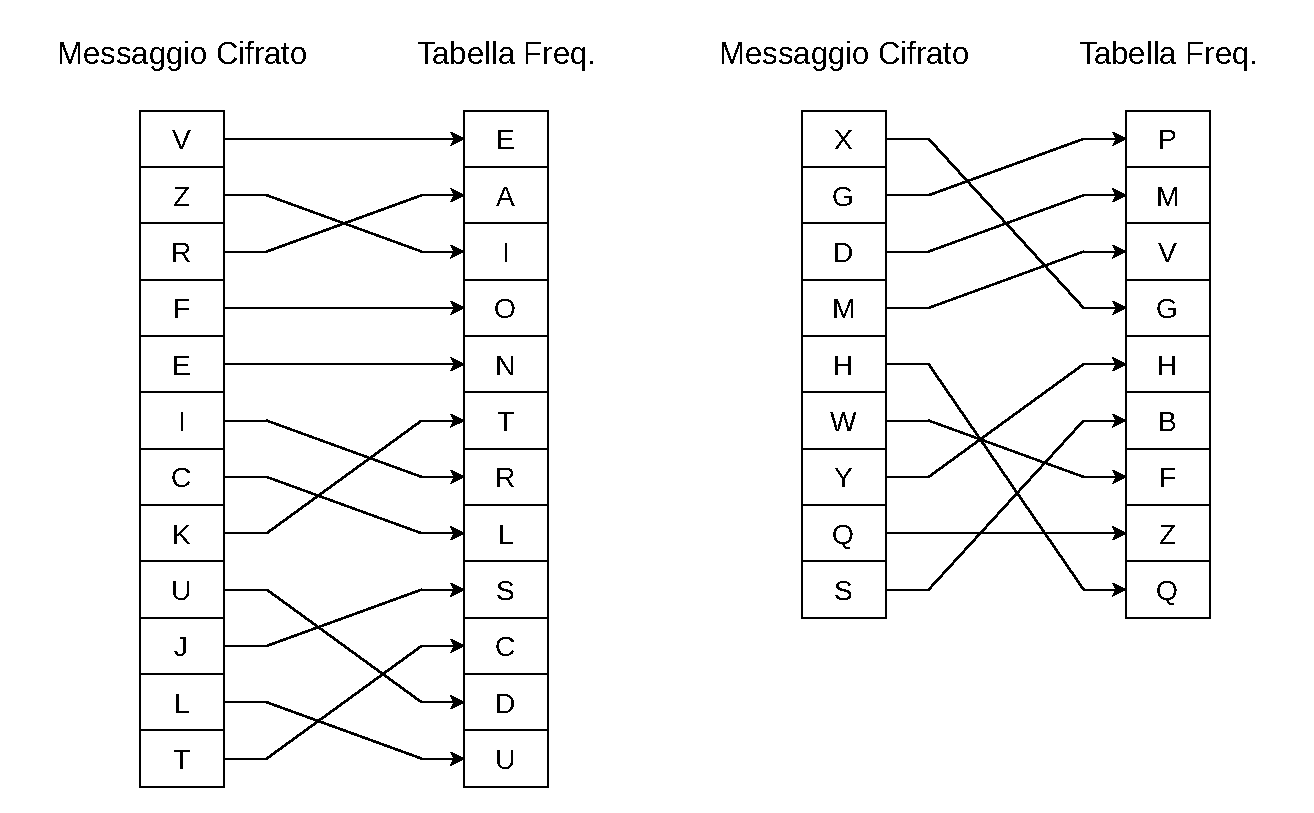
\includegraphics[width=\linewidth]{logos/1_5_cripto.pdf}

\end{figure}

Si può notare che, nel complesso, questa tecnica ha indovinato quasi tutte le lettere; infatti, molte erano sbagliate di una sola posizione.

\begin{itemize}
    \item Indovinate: 4/21 $\approx$ 19.0 \%
    \item Sbagliato di una casella: 10/21 $\approx$ 47.6 \%
    \item Sbagliato di due caselle: 5/21 $\approx$ 23.8 \%
    \item sbagliato di tre caselle: 1/21 $\approx$ 4.8 \%
    \item sbagliato di quattro caselle: 1/21 $\approx$ 4.8 \%
\end{itemize}

\end{document}